\documentclass[margin=3pt]{standalone}
\usepackage[utf8]{inputenc}
\usepackage{tikz}
\usetikzlibrary{arrows,shadows,positioning}

\tikzset{
  frame/.style={
      rectangle, draw, 
      text width=6em, text centered,
      minimum height=4em,drop shadow,fill=gray!20,
      rounded corners,
  },
  line/.style={
    draw, -latex',rounded corners=3mm,
  }
}

\begin{document}

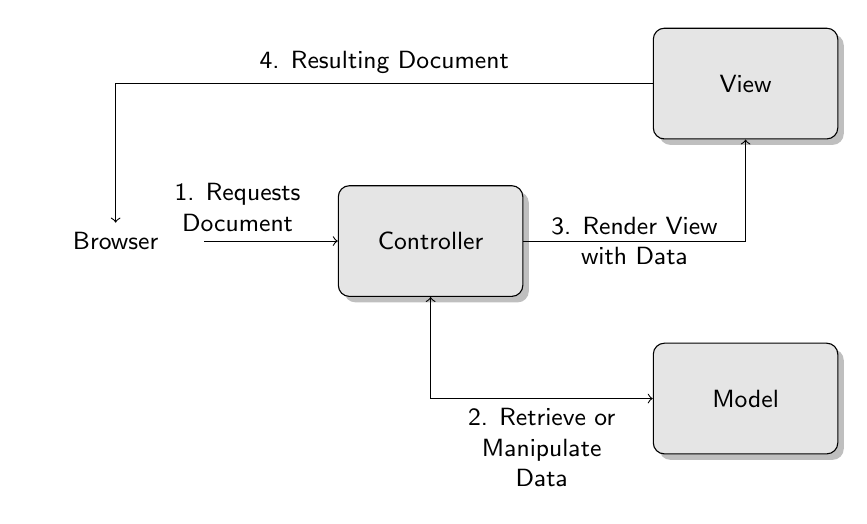
\begin{tikzpicture}[font=\small\sffamily,node distance = 4cm]
\node [frame] (controller) {Controller};
\node [text width=2cm, align=center, left of=controller] (browser) {Browser};
\node [frame, above=2cm, right of=controller] (view) {View};
\node [frame, below=2cm, right of=controller] (model) {Model};

\draw [->] (browser) -- node[above,near start,align=center]{1. Requests\\Document} (controller);
\draw [<->] (controller) |- node[below,align=center,near end] {2. Retrieve or\\Manipulate\\Data} (model);
\draw [->] (controller) -| node[near start, align=center] {3. Render View\\with Data}(view);
\draw [->] (view) -| node[above, pos=.25,align=center]{4. Resulting Document} (browser);
\end{tikzpicture}
\end{document}
